\chapter{Introduction}
\section{Background}
Urban water challenge increases as the cities grow larger. The World Bank estimates that the urban population in worldwide will double by 2050---with serious implications of escalating water demands in cities by 50--70 precent \citep{theworldbankCircularEconomyOpportunity2021}. The amount, distribution, and quality of the available fresh water in urban water cycle has largely been affected by the global climate change. The report from \citep{unicefURBANWATERSCARCITY2021} points out that one in four cities are facing challegnes to supply adequate water to inhabitants, the situation is even worse in cities from developing wrold. Consequently, the rise of urban water usage will also generate more wastewater, thus, the conversion of municipal/industrial wastewater into reusable water is drawing much attentions over the years. Reuse water increases the water availability by substituting the use of freshwater on non-potable (drinkable) uses for agricultural irrigation, industrial, and urban water reuses, etc. 

%%%%%%%%%%%%%%%%%%%%%%%%%%%%
. Costly projects for drinking water supply may also be delayed due to the reduced demand for drinking as a result of reuse. Lastly, reuse is attractive in many communities because the cost of producing treated wastewater has been found to be lower than the cost of producing drinking water. 

In addition, reuse can provide an alternative water supply for many activities that do not require drinking water quality and as such, permit the saved drinking water to be used elsewhere

. \citep{adewumiTreatedWastewaterReuse2010}
%%%%%%%%%%%%%%%%%%%
Wastewater reuse can form an important component of both wastewater management and water resource management and can offer an environmentally sound option for managing wastewater that dramatically reduces environmental impacts associated with the discharge of wastewater to surface waters. 

The construction of reclaimed water facilites often require a huge amount of capital investment. Upgrading available wastewater treatment plants with the reuse water treatment facilities is an economic solution which accompanied with the benefits of the potential of realizing resource recovery (e.g., nitrogen and phosphorus recovery). \citep{maryamWastewaterReclamationReuse2019,kehreinCriticalReviewResource2020}.




The most significant restraints to reuse include the potential risks to public health, and the potential for reduced sewer or stream flows. If implemented under uncontrolled or unregulated circumstances, treated wastewater can be harmful to living beings (if ingested directly or through irrigated crops) and irrigated soil (due to the chemicals and potential bacteria within the effluent)




%paragraph 1 Forecasting models play an important role in water quality control in DTPs and WWTPs.
%paragraph 2 Water reclamation-why is it a good choice for solving urban water scarcity
%paragraph 3 Decision-making processing-how does this help water reclamation
%paragraph 4 Deep learning model to replace fuzzy supervisor and machine learning models-the need of using it
AI technologies have been successfully applied to different DWT processes, such as the prediction of the coagulant 
dosage, discrimination of the DBP formation potential, advanced control of membrane fouling, membrane preparation 
and optimization, and water quality prediction. \cite{liRecentAdvancesArtificial2021}

%%%% Paragraph 1



Forecasting models play an important roles in water quality control in drinking water treatment plants (DTPs) 
and wastewater treatment plants (WWTPs). The need of using forecasting models are becuase the unpredictable 
nature of water quality, and the treatment operations are subjected to the change of water quality to prodcue
effluent complied the government regulation \cite{chenAssessingWastewaterReclamation2003}

%%%% Paragraph 2
Forecasting models can also be called time series model becuase the data is consisted of the values and the 
time (need to be further revised). For the well-know time series models are for example, RNN, ... These are 
used to replace the theory-based models, for example Activated Sludege Model (ASM). The difference between 
these two models are, machine learning based models require to learn from historic data, while the thoery-based
models only need to enter the basic operational parameters (e.g., influent flow, tempearture, and pH, etc).

%%%% Paragraph 3
Despite the promising usage and performance of machine learning models, the collection of the data became
the most difficult tasks. Many small scale or old treatment plants do not have the capital or the available
environment for the set-ups of the online sensors to collect data.
Although these are the major issues, it's still possible to train a forecasting model with one input, which 
is also called a self-prediction model. Although the accuracy or stability compared to multi-input models, 
the forecasted results can be used at some cases. To increase the model performance, there are several ways.
Paper included weather data, or perform data-preprocessing methods to improve the model performance.

%%%% Paragraph 4
These solutions (data preprocessing, feature engineering) are not well discussed in this field, also the 
potential of using univariate models are under estimated.

Keeping an effective disinfectant residual concentration in reclaimed water is still a challenge, due to its high levels of ammonia and organic matter when compared with those in drinking water. \citep{costaIdentificationModellingChlorine2021}


%\begin{figure}[!t]
%   \centering
%   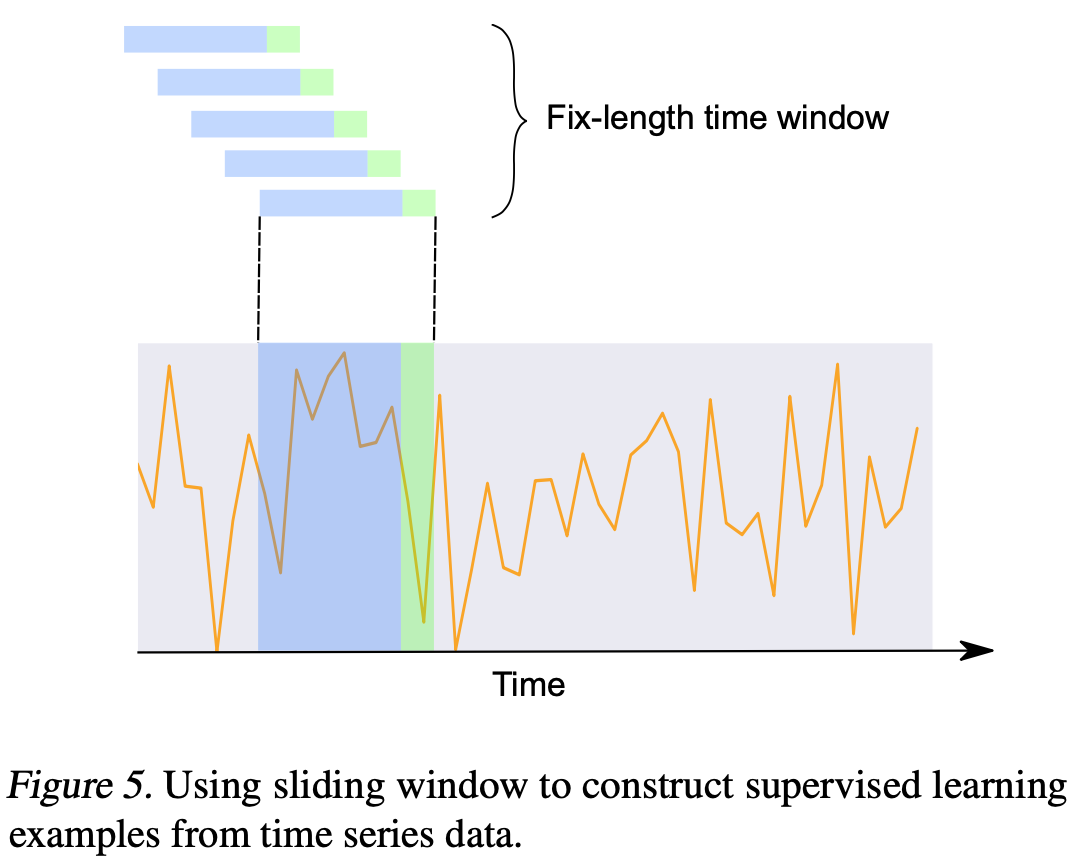
\includegraphics[width=0.75\columnwidth]{imgs/fix-length-time-window.png}
%   \caption{The network structure for the actor-evaluation estimation. It is a combination of convolutional networks for feature extraction and fullyconnected layers for policy learning. They have been separately proven to be effective in our previous works.}
%   \label{fig:ob_network_structure}
%\end{figure}

\section{Objectives}
\noindent
The specific objectives of this thesis work are:\\
%should be investigate the effluent water quality in SWHEPP?
(1) To build baseline univariate forecasting models using machine learning and deep learning models.\\
(2) To develop data preprocessing methods for enhancing model forecasting performance.\\
(3) To extract features and hidden relations of water parameters in MBR effluent by analyzing the wastewater collected upstream of the WWTPs.\\
(4) To develop methods for improving performance of forecasting models using the hidden features and relations of the water parameters.

\section{Organization of the thesis}
In Chapter 1, “Introduction”, the background information, objectives and organization of the thesis were presented.

Chapter 2, “Literature Review”, provides the overview of water quality process controls, the reviews cover the water treatment plant, wastewater treatment plant, and in reclaimed water system.
....

In Chapter 3, “Materials and Methods”, the instruments for ammonia and colour data collection, programming environment, and data preparation methods were summarized. The processes of the formulation of extra features for training forecasting models were illustrated.

In Chapter 4, “Results and discussion”, the performance of machine learning and deep learning models were compared. Forecasting models trained by different data pre-processing methods and the effect of feature engineering were both compared with the baseline model performance. 

In Chapter 5, “Conclusions and Recommendations”, the findings obtained from this thesis work were summarized and the possible future studies were recommended.